% !TEX encoding = UTF-8 Unicode

\level{1}{PDCA} \label{app:pdca}
Il PDCA, acronimo di Plan-Do-Check-Act, conosciuto anche come “Ciclo di Deming” o “Ciclo di miglioramento continuo”, è un modello studiato per il miglioramento continuo della qualità in un'ottica a lungo raggio. Questo strumento parte dall’assunto che per il raggiungimento del massimo della qualità sia necessaria la costante iterazione tra ricerca, progettazione, test e produzione.\\
I miglioramenti ai quali si fa riferimento sono legati all'efficienza e all'efficacia. Migliorare l'efficienza significa usare meno risorse per fare lo stesso lavoro. Migliorare l'efficacia significa divenire più conformi alle aspettative.\\
\begin{figure}[H]
	\centering
	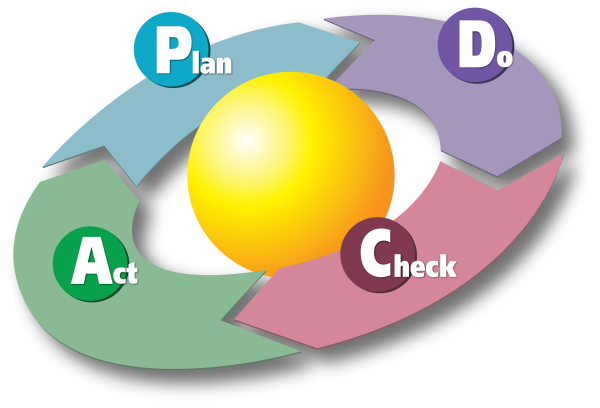
\includegraphics[width=12cm]{PianoDiQualifica/Pics/PDCA_Cycle.png}
	\caption{Ciclo di Deming - PDCA}
\end{figure}
Il ciclo di Deming afferma che affinchè ci possa essere miglioramento continuo ogni processo deve essere dotato di disciplina. In particolare, essi devono seguire le seguenti quattro attività in modo ciclico:
\begin{itemize}
	\item \textbf{Plan - Pianificare}, ovvero definire le attività che si dovranno svolgere, le scadenze che si dovranno rispettare, le responsabilità che si dovranno assegnare e le risorse che si dovranno utilizzare. Prima di eseguire qualsiasi attività si devono pianificare quali sono gli obiettivi di miglioramento, e si deve pensare a come si intende raggiungerli.
	\item \textbf{Do - Eseguire}, cioè eseguire quanto è stato pianificato al punto precedente. Oltre a fare ciò, si devono anche raccogliere i dati necessari all'analisi che viene svolta ai punti successivi.
	\item \textbf{Check - Valutare}, cioè verificare l'esito del processo (per efficienza ed efficacia) rispetto alle attese. In altre parole, si valutano i risultati che si sono ottenuti mettendo in pratica le attività che si sono pianificate in precedenza. I risultati possono avere tre tipi di esito: si è migliorati nel modo atteso, si è fatto meglio o si è fatto peggio.
	\item \textbf{Act - Agire}, cioè applicare soluzioni correttive alle carenze rilevate al punto precedente. Una volta che è stato valutato il risultato ottenuto, e una volta che sono state analizzate le sue carenze, vengono applicate le correzioni.
\end{itemize}
Si noti infine che se si vuole essere migliorabili bisogna essere analizzabili. E per essere analizzabili si deve essere ripetibili. In altre parole: bisogna essere tracciabili, ovvero si devono eseguire le attività facendo si che il modo in cui si ha operato possa essere valutato.